\documentclass[acmtog]{acmart}
\usepackage{graphicx}
\graphicspath{{assets/}}
\usepackage{subfigure}
\usepackage{natbib}
\usepackage{listings}
\usepackage{bm}
\usepackage{amsmath}

\definecolor{blve}{rgb}{0.3372549, 0.61176471, 0.83921569}
\definecolor{gr33n}{rgb}{0.29019608, 0.7372549, 0.64705882}
\makeatletter
\lst@InstallKeywords k{class}{classstyle}\slshape{classstyle}{}ld
\makeatother
\lstset{language=C++,
  basicstyle=\ttfamily,
  keywordstyle=\color{blve}\ttfamily,
  stringstyle=\color{red}\ttfamily,
  commentstyle=\color{magenta}\ttfamily,
  morecomment=[l][\color{magenta}]{\#},
  classstyle = \bfseries\color{gr33n},
  tabsize=2
}
\lstset{basicstyle=\ttfamily}

% Title portion
\title{Assignment 1:\\ {Exploring OpenGL Programming}}

\author{Name:\quad Shu Haoyu \\ student number:\ 2024533012
\\email: \quad \texttt{shuhy2024@shanghaitech.edu.cn}}

% Document starts
\begin{document}
\maketitle

\vspace*{2 ex}

\section{Introduction}
I finished below all tasks using the OpenGL and Arietta math library.
OpenGL is a machine which can remember current status,
modify state according to the input content and state, and can also get the output.

\begin{itemize}
\item Task1:  load mesh objects from files and draw the meshes. 
\item Task1: render objects with a Phong lighting model. 
\item Task2: manipulate the camera using both the keyboard and mouse. Support keyboard controls for translation and rotation, and mouse controls for looking around so that you can navigate the virtual scene.
\item Bonus1:support moving objects in the scene. 
\item Bonus2: support multiple objects in the scene.
\item Bonus3:  support multiple lights in the fragment shader, with different types of lights (such as point lights and spotlights) and different colors. 
\item Bonus4: add a skybox to the scene to make the scene more realistic. 

\end{itemize}
\section{Implementation Details}
\subsection{load mesh objects from files and draw}
I implemented mesh loading and drawing in \texttt{Mesh.cpp}. The constructor \texttt{Mesh(path)} takes the mesh file path as its parameter. I use \texttt{PathOf(target, depth)} to find the file. Here, \texttt{target} is the requested path, and \texttt{depth} is the maximum number of parent-directory levels to search, with a default value of 5. The function returns the absolute file path as a string, or throws an exception if the file cannot be found. Then I open it with \texttt{std::ifstream} and use the input operator \texttt{>{}>} to read the data in order.

First, I read the numbers of positions, normals, and triangles from the beginning of the \texttt{.object} file. I use two temporary vectors to store the positions and normals. Then I read each triangle record, which contains three pairs of position and normal indices. For each pair, I combine the corresponding position and normal into a \texttt{Vertex} and add it to \texttt{vertices\_}. I also store the indices of these new vertices in \texttt{indices\_}. Therefore, each final vertex contains both its position and its normal, although I still need a temporary vector when reading the normals.

I obtain the VAO ID with \texttt{glGenVertexArrays} after loading the data. I create the VBO and EBO IDs with \texttt{glGenBuffers}. Their first parameter is the number of objects to create, and the second is the address where the IDs are stored. I use \texttt{glBindVertexArray} with the VAO ID to select its configuration. I also use \texttt{glBindBuffer}, whose parameters are the buffer target and buffer ID. The VBO uses \texttt{GL\_ARRAY\_BUFFER}, and the EBO uses \texttt{GL\_ELEMENT\_ARRAY\_BUFFER}.

I upload the data with \texttt{glBufferData}. Its four parameters are the buffer target, the data size in bytes, the address of the data, and a usage hint. For the vertices, I use \texttt{vertices\_.size()} multiplied by \texttt{sizeof(Vertex)} as the byte size. For the triangle indices, I use the number of stored index triples multiplied by the size of one triple. I choose \texttt{GL\_STATIC\_DRAW} because the uploaded mesh data stays unchanged while the program runs.

Then I describe the vertex layout with \texttt{glVertexAttribPointer}. Its parameters are the attribute location, number of components, component type, integer normalization flag, stride in bytes, and offset in the VBO. I use location 0 for the position and location 1 for the normal. Both have three \texttt{GL\_FLOAT} components, with \texttt{GL\_FALSE} for integer normalization and \texttt{sizeof(Vertex)} as the stride. The position offset is zero. For the normal, I use \texttt{offsetof} with \texttt{Vertex} and its \texttt{normal} member to get the offset. Finally, \texttt{glEnableVertexAttribArray} takes an attribute location and enables it. The VAO records these settings and the associated buffers.

In \texttt{Main()}, I create a \texttt{Mesh} object by passing the file path to its constructor. In the rendering loop, I call its \texttt{Draw()} function, which has no parameters. It binds the VAO and calls \texttt{glDrawElements}. The four arguments specify the primitive type, number of scalar indices, index type, and byte offset in the EBO. I use \texttt{GL\_TRIANGLES}, three indices per stored triangle, \texttt{GL\_UNSIGNED\_INT}, and offset 0. The mesh file is loaded once, rather than read again in every frame.

Before drawing a frame, I call \texttt{glClearColor} with red, green, blue, and alpha values to set the clear color. Then \texttt{glClear} takes a mask containing \texttt{GL\_COLOR\_BUFFER\_BIT} and \texttt{GL\_DEPTH\_BUFFER\_BIT} to clear both buffers. I present the frame with \texttt{glfwSwapBuffers}. Its single parameter identifies the window whose back buffer is presented.
\subsection{render objects with a Phong lighting model}
I use \texttt{model.vert} and \texttt{model.frag} for Phong lighting. The constructor \texttt{Shader(vsPath, fsPath)} takes the paths of the vertex and fragment shader files. In \texttt{Shader.cpp}, I use \texttt{glCreateShader} with a shader type to create each shader. Then \texttt{glShaderSource} receives the shader ID, number of source strings, address of the source-string pointer, and source lengths. I pass one string and use \texttt{nullptr} for the lengths because the string is null-terminated. I call \texttt{glCompileShader} with the shader ID to compile it.

Next, I call \texttt{glCreateProgram}, which takes no parameters and returns a program ID. I use \texttt{glAttachShader} with the program ID and shader ID, and then \texttt{glLinkProgram} with the program ID. I check compilation with \texttt{glGetShaderiv} and \texttt{GL\_COMPILE\_STATUS}, and linking with \texttt{glGetProgramiv} and \texttt{GL\_LINK\_STATUS}. These queries take an object ID, the property to query, and a pointer for the result. If a step fails, I use \texttt{glGetShaderInfoLog} or \texttt{glGetProgramInfoLog} to read its diagnostic log. Their parameters are the object ID, output buffer size, an optional pointer for the written length, and the output buffer. Then I throw an exception.

Before setting uniforms, I call \texttt{Shader::Use()}, which activates the program through \texttt{glUseProgram}. I pass uniforms through \texttt{Shader::Set}. Its parameters are \texttt{name} and \texttt{value}: the uniform name and the value to upload. I use it for the matrices, camera position, material color, and lighting parameters. The member function \texttt{GetUniformLocation} takes a uniform name and finds its location using the program ID and that name. The \texttt{Set} overload chooses the corresponding uniform function. For example, \texttt{glUniformMatrix4fv} takes the location, matrix count, transpose flag, and data pointer. I pass one matrix with \texttt{GL\_FALSE} to upload it without transposing it.

First, the vertex shader uses the model matrix to transform the vertex position into world space. It then applies the view and projection matrices to obtain the clip-space position. I also transform the normal using the upper-left three-by-three part of the model matrix. This works for the translations and positive uniform scaling used in my scene, after normalization in the fragment shader. Non-uniform scaling would require an inverse-transpose normal matrix.

\paragraph{The MVP transformation.}
I use column vectors and a right-handed coordinate system. A local vertex is written as the homogeneous point $\mathbf p_o=(x,y,z,1)^{\mathsf T}$. The last component is 1 for a point and 0 for a direction, so translation changes points but not directions. The three matrices act in this order:
\begin{equation}
\begin{aligned}
\mathbf p_w&=M\mathbf p_o,\\
\mathbf p_v&=V\mathbf p_w,\\
\mathbf p_c&=P\mathbf p_v=PVM\mathbf p_o.
\end{aligned}
\end{equation}
Here, the subscripts mean object, world, view, and clip space. Although I call this the MVP transformation, the product in my shader is $PVM$, because the rightmost matrix acts first. After clipping, perspective division gives normalized device coordinates (NDC):
\begin{equation}
\mathbf p_{\mathrm{ndc}}=
\left(\frac{x_c}{w_c},\frac{y_c}{w_c},\frac{z_c}{w_c}\right).
\end{equation}
The viewport then maps these coordinates to the window. Therefore, the output of $PVM$ is a clip-space point, and it still needs division by $w_c$ before the viewport mapping.

Then the fragment shader receives the interpolated world position and normal. I normalize the normal, the direction from the surface to the light, and the direction from the surface to the camera. All these quantities are in world space, so I can use them together in the lighting calculation.

The Phong model has three parts: ambient, diffuse, and specular lighting. The ambient part gives the object a basic color even when it does not face a light, with \texttt{ka} controlling its strength. For the diffuse part, I use \texttt{dot(N, L)} to calculate the dot product of the unit normal and the direction toward the light. I use \texttt{max} with zero to remove negative values. For the specular part, \texttt{reflect(-L, N)} returns the reflected direction, where \texttt{-L} is the incoming direction and \texttt{N} is the unit normal. I compare this result with the viewing direction and use \texttt{pow} to raise the nonnegative dot product to \texttt{s}. Its first argument is the base, and its second is the exponent. The coefficient \texttt{ks} controls the highlight strength, and \texttt{s} controls how concentrated it is. I also set the specular contribution to zero when the surface faces away from the light. Finally, I add the lighting contributions to get the fragment color.

For a world-space surface point $\mathbf x$, light position $\mathbf l_j$, and camera position $\mathbf e$, I use unit vectors
\begin{equation}
\boldsymbol\ell_j=\frac{\mathbf l_j-\mathbf x}{\|\mathbf l_j-\mathbf x\|},
\qquad
\mathbf v=\frac{\mathbf e-\mathbf x}{\|\mathbf e-\mathbf x\|}.
\end{equation}
I assume these differences are nonzero. Since the normal $\mathbf n$ is also a unit vector, $\mathbf n\cdot\boldsymbol\ell_j$ is the cosine of the angle toward the light. This gives the diffuse factor. Reflecting the incoming vector $-\boldsymbol\ell_j$ across the surface gives
\begin{equation}
\begin{aligned}
d_j&=\max(\mathbf n\cdot\boldsymbol\ell_j,0),\\
\boldsymbol\rho_j&=2(\mathbf n\cdot\boldsymbol\ell_j)\mathbf n-\boldsymbol\ell_j,\\
h_j&=
\begin{cases}
[\max(\boldsymbol\rho_j\cdot\mathbf v,0)]^s,&d_j>0,\\
0,&d_j=0.
\end{cases}
\end{aligned}
\end{equation}
Thus, the color returned by \texttt{light} is
\begin{equation}
F_j=d_j(\mathbf C_j\odot\mathbf C_m)+k_s h_j\mathbf C_j.
\end{equation}
Here, $\mathbf C_j$ is the light color, $\mathbf C_m$ is the material color, and $\odot$ means component-wise RGB multiplication. The exponent $s$ is the Phong shininess value, rather than the scale factor used by \texttt{scale}. This is the Phong lighting model used in my shader.
\subsection{manipulate the camera using both the keyboard and mouse}
I implemented camera control in \texttt{Main.cpp} and use the functions in \texttt{Math.cpp} to build the required matrices. I store the camera position in \texttt{eye} and its viewing direction in \texttt{direction}. I process input events with \texttt{glfwPollEvents}, which takes no parameters. To check a key, I use \texttt{glfwGetKey(window, key)}. Its parameters identify the window and key, and I compare the result with \texttt{GLFW\_PRESS}. I also use \texttt{glfwGetTime()}, which returns elapsed time in seconds, to calculate the time between frames.

For translation, W and S move the camera along its viewing direction. A and D move it sideways. I use \texttt{direction.Cross(up)} to obtain the cross product of the viewing direction and world up vector, and divide it by its \texttt{Norm()} to obtain a unit right vector. Space and Left Ctrl move the camera up and down along the world vertical axis. I multiply the movement speed by the time between frames, so the displacement depends on elapsed time rather than the number of frames.

For rotation, Q and E change yaw, while Z and C change pitch. I register \texttt{MouseCallback} through \texttt{glfwSetCursorPosCallback}, passing the window and callback function. The callback receives \texttt{window}, \texttt{xpos}, and \texttt{ypos}; the last two are cursor coordinates in the window's content area. I compare them with the previous coordinates to obtain the movement. I multiply this movement by a sensitivity value and add it to yaw and pitch. The first callback only records the mouse position, which avoids a sudden change when mouse control starts. I limit pitch to $[-89^\circ,89^\circ]$ to avoid looking exactly along the world up axis. I use \texttt{glfwSetInputMode} with the window, \texttt{GLFW\_CURSOR}, and \texttt{GLFW\_CURSOR\_DISABLED} to hide and capture the cursor.

In each frame, I rebuild the viewing direction from the initial forward vector and the stored angles. I use \texttt{rotate(theta, axis)}, which returns a four-by-four rotation matrix. Here, \texttt{theta} is an angle in degrees, and \texttt{axis} is the rotation axis, which the function normalizes internally. I use the three-by-three rotation part for the direction vector. Yaw rotates it around the world up axis, and pitch rotates it around the current right axis.

\paragraph{Deriving \texttt{rotate}.}
First, I convert the input angle to radians, $\theta_r=\theta\pi/180$, and normalize the nonzero axis to $\mathbf a$. To rotate a vector $\mathbf b$, I split it into a part along the axis and a part perpendicular to it:
\begin{equation}
\mathbf b_\parallel=\mathbf a(\mathbf a\cdot\mathbf b),
\qquad
\mathbf b_\perp=\mathbf b-\mathbf b_\parallel.
\end{equation}
The parallel part stays unchanged. The perpendicular part rotates in its plane, where $\mathbf a\times\mathbf b$ gives the second perpendicular direction. Therefore,
\begin{equation}
\mathbf b'=\mathbf b_\parallel+
\cos\theta_r\,\mathbf b_\perp+
\sin\theta_r\,(\mathbf a\times\mathbf b).
\end{equation}
After substituting the two parts and collecting terms, I obtain Rodrigues' rotation matrix:
\begin{equation}
R=\cos\theta_r I+(1-\cos\theta_r)\mathbf a\mathbf a^{\mathsf T}
+\sin\theta_r[\mathbf a]_\times,
\end{equation}
\begin{equation}
[\mathbf a]_\times=
\begin{pmatrix}
0&-a_z&a_y\\
a_z&0&-a_x\\
-a_y&a_x&0
\end{pmatrix}.
\end{equation}
This matrix satisfies $[\mathbf a]_\times\mathbf b=\mathbf a\times\mathbf b$. In my code, \texttt{First}, \texttt{Second}, and \texttt{Third} are the three terms of $R$. I put $R$ in the upper-left part of a four-by-four identity matrix. The angle follows the right-hand rule; when $\theta=0$, the result is the identity matrix.

For yaw $\psi$ and pitch $\phi$, the direction update can be written as
\begin{equation}
\begin{aligned}
\mathbf d_y&=R(\psi,\mathbf u_0)\mathbf d_0,\\
\mathbf r_y&=\frac{\mathbf d_y\times\mathbf u_0}{\|\mathbf d_y\times\mathbf u_0\|},\\
\mathbf d&=R(\phi,\mathbf r_y)\mathbf d_y.
\end{aligned}
\end{equation}
Here, $\mathbf d_0=(0,0,-1)$ is the initial forward direction and $\mathbf u_0=(0,1,0)$ is world up. This matches my order of yaw first and pitch second. Rotations preserve vector length, so the direction remains unit length in exact arithmetic.

Finally, I call \texttt{lookAt(eye, center, up)} to update the view matrix. The parameters are the camera position, a world-space point to look at, and a reference up vector. In my call, \texttt{center} is the point \texttt{eye + direction}, rather than the direction alone. I also use \texttt{perspective} with \texttt{fovY}, \texttt{aspect}, \texttt{nearplane}, and \texttt{farplane} to obtain the projection matrix. These parameters are the vertical field of view in degrees, window width divided by height, and positive distances to the near and far clipping planes. My settings are $50^\circ$, $1280/720$, $0.1$, and $100$. Changing the view matrix changes the camera view without modifying the mesh data.

\paragraph{Deriving \texttt{lookAt}.}
I use $\mathbf e$ for \texttt{eye}, $\mathbf c$ for the target \texttt{center}, and $\mathbf u_0$ for the reference up vector. First, I build the camera's forward, right, and corrected up directions:
\begin{equation}
\begin{aligned}
\mathbf f&=\frac{\mathbf c-\mathbf e}{\|\mathbf c-\mathbf e\|},\\
\mathbf r&=\frac{\mathbf f\times\mathbf u_0}{\|\mathbf f\times\mathbf u_0\|},\\
\mathbf u&=\frac{\mathbf r\times\mathbf f}{\|\mathbf r\times\mathbf f\|}.
\end{aligned}
\end{equation}
The target must differ from the eye, and the reference up vector must not be parallel to the forward direction. My function checks these cases before dividing. The camera's positive Z axis is $-\mathbf f$, so points in front of it have negative view-space Z.

Then I subtract the camera position from a world point $\mathbf x$. Its camera coordinates are the projections of $\mathbf x-\mathbf e$ onto the three camera axes:
\begin{equation}
\begin{aligned}
x_v&=\mathbf r\cdot(\mathbf x-\mathbf e),\\
y_v&=\mathbf u\cdot(\mathbf x-\mathbf e),\\
z_v&=-\mathbf f\cdot(\mathbf x-\mathbf e).
\end{aligned}
\end{equation}
Expanding these dot products gives the view matrix:
\begin{equation}
V=
\begin{pmatrix}
r_x&r_y&r_z&-\mathbf r\cdot\mathbf e\\
u_x&u_y&u_z&-\mathbf u\cdot\mathbf e\\
-f_x&-f_y&-f_z&\mathbf f\cdot\mathbf e\\
0&0&0&1
\end{pmatrix}.
\end{equation}
The vectors \texttt{v1} through \texttt{v4} in my function store its four columns. As a check on the formula, the eye maps to $(0,0,0,1)$, and the point $\mathbf e+\mathbf f$ maps to $(0,0,-1,1)$.

\paragraph{Deriving \texttt{perspective}.}
I write $n$ and $f$ for the positive near and far distances, with $0<n<f$, and $a$ for the aspect ratio. Let $\alpha=\texttt{fovY}\,\pi/180$, with $0<\alpha<\pi$. From the right triangle between the eye and the top of the near plane, its half-height is $h=n\tan(\alpha/2)$ and its half-width is $ah$.

For a view-space point $(x_v,y_v,z_v)$ in front of the camera, its positive depth is $d=-z_v$. Similar triangles give $x_{\mathrm{near}}=nx_v/d$ and $y_{\mathrm{near}}=ny_v/d$. Dividing by the near-plane half-width and half-height gives
\begin{equation}
x_{\mathrm{ndc}}=\frac{q x_v}{a d},
\qquad
y_{\mathrm{ndc}}=\frac{q y_v}{d},
\end{equation}
where $q=1/\tan(\alpha/2)$. I can obtain these expressions by setting $x_c=qx_v/a$, $y_c=qy_v$, and $w_c=-z_v=d$, then dividing by $w_c$.

Next, I choose $z_c=Az_v+B$. OpenGL's NDC depth should be $-1$ on the near plane and $+1$ on the far plane. Substituting $z_v=-n$ and $z_v=-f$ gives
\begin{equation}
\begin{aligned}
\frac{-An+B}{n}&=-1,\\
\frac{-Af+B}{f}&=1.
\end{aligned}
\end{equation}
Thus, $B=An-n=Af+f$. Solving these two equations gives
\begin{equation}
A=-\frac{f+n}{f-n},
\qquad B=-\frac{2fn}{f-n}.
\end{equation}
Combining the X, Y, Z, and W expressions gives the matrix returned by my function:
\begin{equation}
P=
\begin{pmatrix}
q/a&0&0&0\\
0&q&0&0\\
0&0&-\dfrac{f+n}{f-n}&-\dfrac{2fn}{f-n}\\[4pt]
0&0&-1&0
\end{pmatrix}.
\end{equation}
The variable \texttt{s} inside \texttt{perspective} stores $q$; it is separate from the Phong exponent. Substituting the near and far depths into this matrix gives $z_{\mathrm{ndc}}=-1$ and $+1$, respectively. Under the default depth mapping, the depth-buffer value is $(z_{\mathrm{ndc}}+1)/2$, so these planes map to 0 and 1.
\subsection{support moving objects in the scene.}
I use the center of the screen to select an object. A small crosshair shows the aiming position, and the picking ray starts at \texttt{eye} and follows \texttt{direction}. I use \texttt{glfwSetMouseButtonCallback} to register the mouse-button callback. Its arguments identify the window and the callback function, \texttt{MouseButtonCallback}. The callback parameters are \texttt{window}, \texttt{button}, \texttt{action}, and \texttt{mods}. They identify the window, mouse button, press or release action, and modifier-key flags. I check the left button and use the action to record its press and release.

I draw the crosshair with \texttt{glDrawArrays}. Its parameters are the primitive type, first vertex index, and vertex count; I use \texttt{GL\_POINTS}, 0, and 1. The crosshair shader puts this point at the screen center, and \texttt{glPointSize(3.0f)} sets its size to 3 pixels. I temporarily call \texttt{glDisable} with \texttt{GL\_DEPTH\_TEST}, so the crosshair is drawn over the scene, and enable the test again afterward.

When the button is pressed, I call \texttt{OnSphere} with \texttt{eye}, \texttt{direction}, \texttt{R}, and \texttt{center}. The first two parameters define the world-space ray, and the last two specify the sphere radius and center. The function returns the nearest valid positive ray parameter \texttt{t}, or zero when there is no valid forward hit. This parameter is a distance only when the input direction is a unit vector. I use a radius of 2.55 for each sphere and 2.19 for the bunny's sphere proxy. The bunny uses this proxy rather than exact triangle intersections, so its selectable region can extend beyond its visible outline.

To obtain the sphere intersection, I write the ray as $\mathbf x(t)=\mathbf e+t\mathbf d$, where $\mathbf d$ is the nonzero input direction. For sphere center $\mathbf c$ and radius $R>0$, I substitute this ray into $\|\mathbf x-\mathbf c\|^2=R^2$. With $\mathbf v=\mathbf e-\mathbf c$, expansion gives
\begin{equation}
(\mathbf d\cdot\mathbf d)t^2+
2(\mathbf v\cdot\mathbf d)t+
\mathbf v\cdot\mathbf v-R^2=0.
\end{equation}
Let $l=\|\mathbf d\|$, $m=\|\mathbf v\|$, and $\cos\beta=(\mathbf v/m)\cdot(\mathbf d/l)$ when $m>0$. The same quadratic can be solved as
\begin{equation}
\Delta=R^2-m^2(1-\cos^2\beta),
\qquad t_\pm=\frac{-m\cos\beta\pm\sqrt{\Delta}}{l}.
\end{equation}
Here, $m\sin\beta$ is the perpendicular distance from the center to the ray's line. A negative $\Delta$ means the line misses the sphere; otherwise, I choose the smallest positive root. The division by $l$ keeps $t$ consistent with the original input direction. If the eye is at the center, my function handles it separately with $t=R/l$. It also uses a small tolerance around $\Delta=0$ for near-tangent cases.

For the plane, I call \texttt{OnPlane} with \texttt{eye}, \texttt{direction}, \texttt{R}, \texttt{center}, and \texttt{normal}. Here, \texttt{R} is the square's half-size, rather than a sphere radius, and \texttt{normal} is the plane normal. I use a half-size of 1 and the normal $(0,0,1)$. The function returns a positive ray parameter when the intersection is in front of the camera and inside the square, and zero otherwise. Its X and Y boundary checks are intended for my current plane orientation.

For the plane equation $\mathbf n\cdot(\mathbf x-\mathbf c)=0$, substituting the same ray gives
\begin{equation}
\begin{aligned}
\mathbf n\cdot(\mathbf e+t\mathbf d-\mathbf c)&=0,\\
t&=\frac{\mathbf n\cdot(\mathbf c-\mathbf e)}{\mathbf n\cdot\mathbf d}.
\end{aligned}
\end{equation}
I reject a denominator close to zero because the ray is parallel to the plane. Then I require $t>0$ and check the hit point against $|x-c_x|\leq R$ and $|y-c_y|\leq R$. These square bounds apply to my plane parallel to the world XY plane.

Then I collect the returned parameters in a vector and pass it to \texttt{nearestHitIndex}. Its argument, \texttt{distances}, is this vector of candidate ray parameters. The function returns the index of the smallest positive value, or $-1$ if no valid hit exists. All candidates use the same ray, so I can compare these values to select the closest object.

After selecting an object, I transform its center from world space into camera space and save this position in \texttt{objectCatchPosition}. While the button remains held, I keep this saved position fixed and call \texttt{V.Inverse()}. This member function takes no parameters and returns the inverse of the current view matrix. I multiply it by the saved camera-space position to obtain the new world position. Then I update the selected object's position and model matrix. This makes the object keep the same position relative to the camera when I move or turn.

If $V_0$ is the view matrix when I select the object and $\mathbf p_{w,0}$ is its homogeneous world-space center, the saved point is $\mathbf q=V_0\mathbf p_{w,0}$. For the current frame $k$, I update it by
\begin{equation}
\mathbf p_{w,k}=V_k^{-1}\mathbf q,
\qquad V_k\mathbf p_{w,k}=\mathbf q.
\end{equation}
The second equality shows why dragging works: the center stays at the saved camera-space coordinates. Since the projection matrix stays fixed, its projected screen position and view-space depth also stay fixed.

The selected object stays selected until I release the button. On release, I clear the selection and leave the object at its new world position. This operation changes the object's position, but does not rotate its orientation with the camera.
\subsection{ support multiple objects in the scene.}
I create separate \texttt{Mesh} instances for two spheres, a bunny, and a plane in \texttt{Main()}. The two spheres load the same mesh file, but have separate positions. I also use an \texttt{Object} structure to store each object's local center, world position, and scale.

In each frame, I set a different model matrix before drawing each object. I use \texttt{translation(pos, center)}, which returns a four-by-four matrix that moves the first point to the second point. Its displacement is \texttt{center - pos}; despite the parameter names, \texttt{pos} is the source point and \texttt{center} is the destination. For the spheres and plane, I pass the object's local center and current world position.

For the bunny, I first call \texttt{translation} to move its local center to the origin. Then I use \texttt{scale(s)}, whose single parameter is a uniform scale factor, to obtain a four-by-four scaling matrix. Finally, another translation moves the origin to the bunny's world position. I use a factor of 20. This order allows me to scale the bunny around the chosen center. Before each draw, I use \texttt{shader.Set} with the uniform name \texttt{M} and that object's model matrix.

\paragraph{Deriving the model matrix.}
For \texttt{translation(pos, center)}, let the input points be $\mathbf a$ and $\mathbf b$. The required displacement is $\boldsymbol\delta=\mathbf b-\mathbf a$, because $\mathbf a+\boldsymbol\delta=\mathbf b$. I place this displacement in the last column:
\begin{equation}
T(\boldsymbol\delta)=
\begin{pmatrix}
1&0&0&\delta_x\\
0&1&0&\delta_y\\
0&0&1&\delta_z\\
0&0&0&1
\end{pmatrix}.
\end{equation}
Then $T(\boldsymbol\delta)(\mathbf x,1)^{\mathsf T}=(\mathbf x+\boldsymbol\delta,1)^{\mathsf T}$. Uniform scaling multiplies each spatial coordinate by the factor $s$, while preserving the homogeneous component:
\begin{equation}
S(s)=
\begin{pmatrix}
s&0&0&0\\
0&s&0&0\\
0&0&s&0\\
0&0&0&1
\end{pmatrix}.
\end{equation}
For local center $\mathbf c$ and desired world position $\mathbf p$, the bunny's model matrix is
\begin{equation}
M=T(\mathbf p)S(s)T(-\mathbf c).
\end{equation}
Applying the matrices from right to left gives
\begin{equation}
\mathbf x_w=s(\mathbf x_o-\mathbf c)+\mathbf p.
\end{equation}
This is why I use \texttt{BunnyT2 * BunnyS * BunnyT1}. The center $\mathbf x_o=\mathbf c$ maps exactly to $\mathbf p$, regardless of the scale. For the spheres and plane, $s=1$, so the model matrix reduces to $T(\mathbf p-\mathbf c)$.

All these objects use the same model shader, view matrix, and projection matrix. Their separate model matrices place them at different positions. I call \texttt{glEnable} with \texttt{GL\_DEPTH\_TEST} to enable depth testing, so the visible surfaces are determined by their depth rather than only by the order of drawing.

\subsection{support multiple lights in the fragment shader}
I use one point light and one spotlight, with different colors. I define their parameters in \texttt{Main.cpp} and send them to the fragment shader through \texttt{Shader::Set}. The uniforms \texttt{pointPosition} and \texttt{pointColor} describe the point light's world position and RGB color. For the spotlight, \texttt{glightPosition}, \texttt{gColor}, and \texttt{gDirection} describe its position, RGB color, and direction from the light toward the cone. The uniform \texttt{gCosCutoff} stores the cosine of the cone's half-angle. I compute it with \texttt{std::cos}, which takes an angle in radians, so I convert $30^\circ$ to radians first.

I use the same \texttt{light} function in \texttt{model.frag} for both lights. Its five parameters are \texttt{lightPosition}, \texttt{lightColor}, \texttt{worldPosition}, \texttt{N}, and \texttt{V}. They represent the light's world position and RGB color, the fragment's world position, the unit normal, and the unit direction from the fragment to the camera. This \texttt{V} is a direction vector inside the function, rather than the view matrix used by the vertex shader. The function returns a three-component color containing diffuse and specular contributions. It also uses the uniforms \texttt{material}, \texttt{ks}, and \texttt{s}.

For the spotlight, I use \texttt{normalize} to obtain unit directions and \texttt{dot} to compare the spotlight direction with the direction from the light to the fragment. If the cosine of their angle is greater than or equal to \texttt{gCosCutoff}, the fragment is inside the light cone. Otherwise, the spotlight contributes zero.

Finally, I add the point-light and spotlight contributions to the ambient term. I add ambient lighting only once, rather than once for each light. My spotlight has a half-angle of $30^\circ$ and stays at a fixed world position. This version uses a hard cutoff at the cone boundary and does not include distance attenuation.
\subsection{ add a skybox}
I implemented cubemap loading in \texttt{Texture.cpp}. The constructor \texttt{Texture(paths)} takes a vector containing exactly six image paths, in positive X, negative X, positive Y, negative Y, positive Z, and negative Z order. I create a texture ID with \texttt{glGenTextures}, whose parameters are the number of textures and the address for storing their IDs. Then I use \texttt{glBindTexture} with \texttt{GL\_TEXTURE\_CUBE\_MAP} and the texture ID to select the cubemap.

For each face, I call \texttt{Texture::Load(path, target)}. Its parameters are the image path and the cubemap face to fill. Inside this function, \texttt{stbi\_load} takes the image filename, pointers for width, height, and the original channel count, and the requested output channel count. I pass \texttt{STBI\_rgb} to obtain three-channel RGB data. The function returns a pointer to the decoded pixels, or a null pointer if loading fails.

I upload the pixels with \texttt{glTexImage2D}. Its arguments specify the face target, mipmap level, internal GPU format, width, height, border, input pixel format, component type, and pixel pointer. I use level 0, \texttt{GL\_RGB8}, the loaded dimensions, border 0, \texttt{GL\_RGB}, and \texttt{GL\_UNSIGNED\_BYTE}. After uploading, I pass the pixel pointer to \texttt{stbi\_image\_free} to release the CPU image data.

I set sampling parameters with \texttt{glTexParameteri}. Its three parameters are the texture target, parameter name, and parameter value. I use \texttt{GL\_LINEAR} for the minification and magnification filters, and \texttt{GL\_CLAMP\_TO\_EDGE} for the S, T, and R wrapping modes. In \texttt{Main.cpp}, \texttt{glActiveTexture} with \texttt{GL\_TEXTURE0} selects texture unit 0. I call \texttt{Texture::Bind()}, which has no parameters and binds this texture to the cubemap target. Then I set \texttt{skyboxTexture} to integer 0 through \texttt{Shader::Set}. This value is the texture-unit index, rather than the texture object ID.

I draw a cube(which is created by myself) as the skybox. In \texttt{skybox.vert}, I use \texttt{mat3(V)} to keep the rotation part of the view matrix and convert it back to a four-by-four matrix with \texttt{mat4}. This removes the translation. Therefore, turning the camera changes the visible background direction, while translating the camera does not shift the background as if it were a nearby object. In the fragment shader, \texttt{texture} takes the cubemap sampler and \texttt{sampleDirection} and returns the sampled color. The direction comes from the cube's local position.

I draw the skybox after the scene objects. In the vertex shader, I set the clip-space Z component equal to W, which places the skybox at the farthest depth after perspective division. During this draw, I call \texttt{glDepthFunc} with \texttt{GL\_LEQUAL}. Its parameter selects the comparison rule, and this rule accepts a depth less than or equal to the stored depth. Depth testing stays enabled, so the scene objects can still cover the background. I also call \texttt{glDepthMask} with \texttt{GL\_FALSE} to disable depth writes. Its boolean parameter controls writing, rather than testing. After drawing, I restore \texttt{GL\_LESS} and enable depth writes with \texttt{GL\_TRUE}.
\section{Results}
The six images below show the combined lighting effects of the spotlight and point light. I show the scene from different viewing angles to compare the lighting effects. The images also show how the different light colors mix on the object surfaces and how the skybox provides the background of the scene.
The blue is come from point light and the red is come from spotlight light.
\begin{figure}[h]
	\centering
	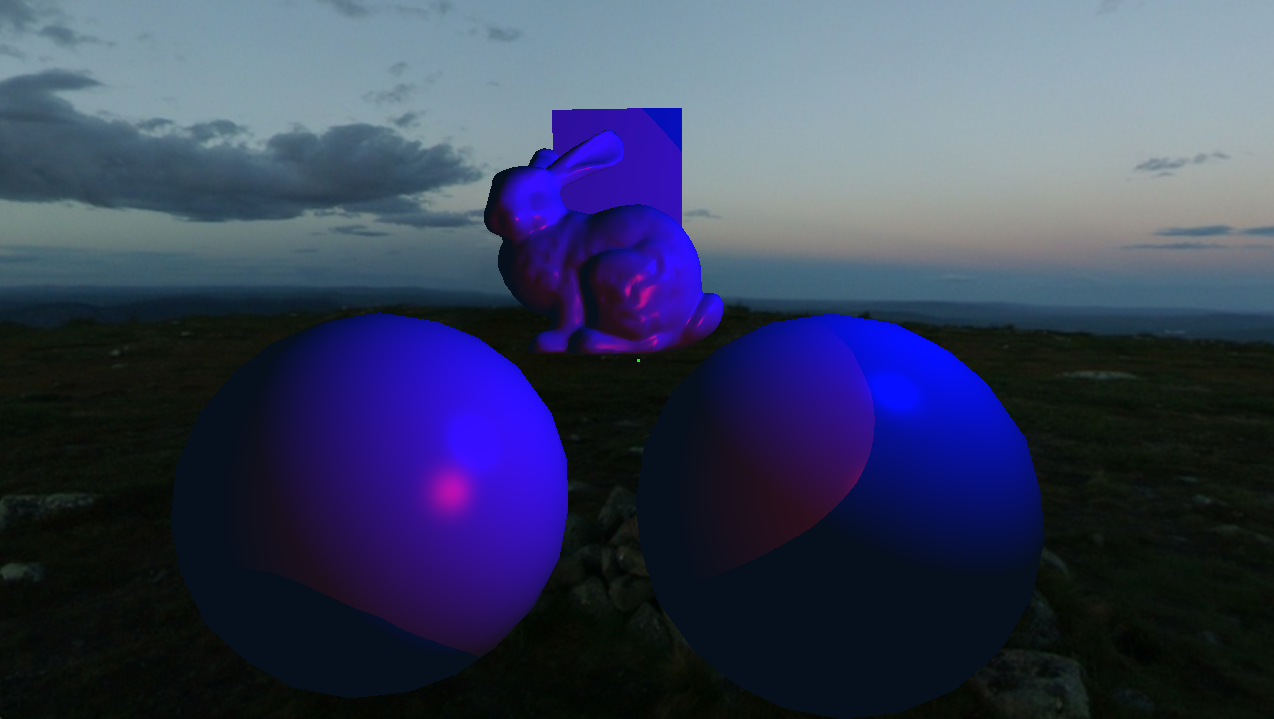
\includegraphics[width=0.48\linewidth]{1}
	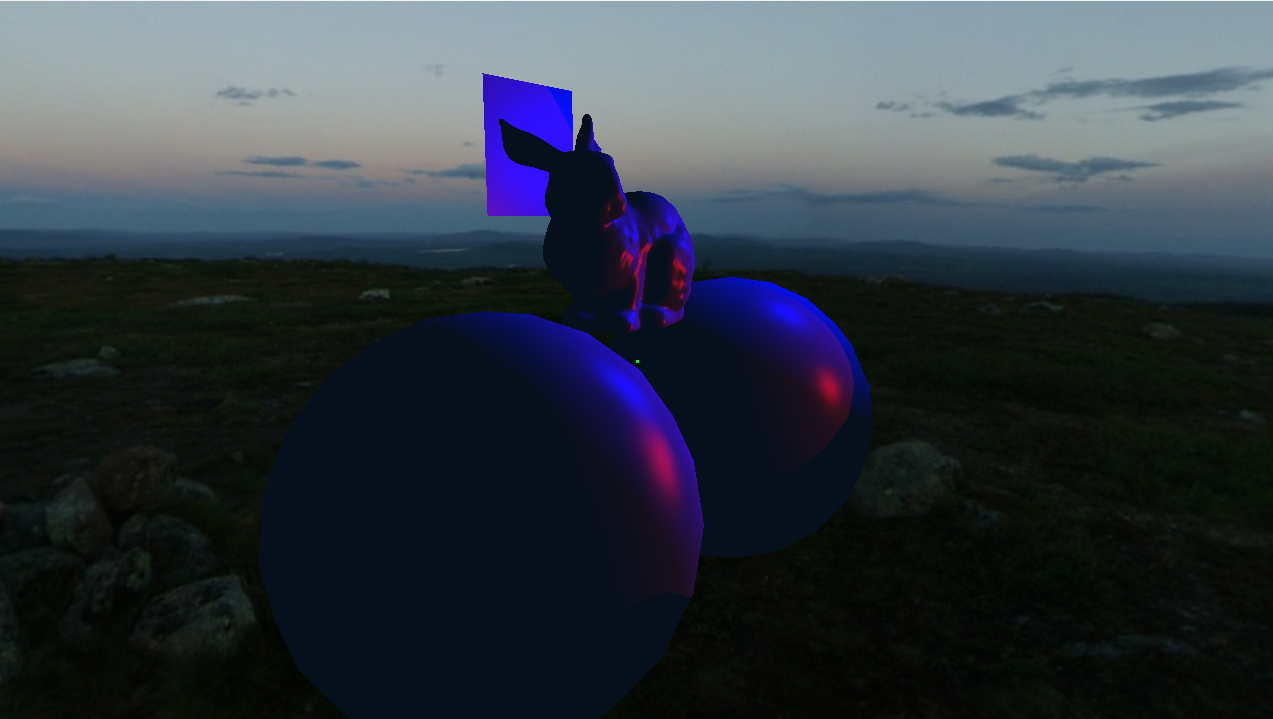
\includegraphics[width=0.48\linewidth]{2}
	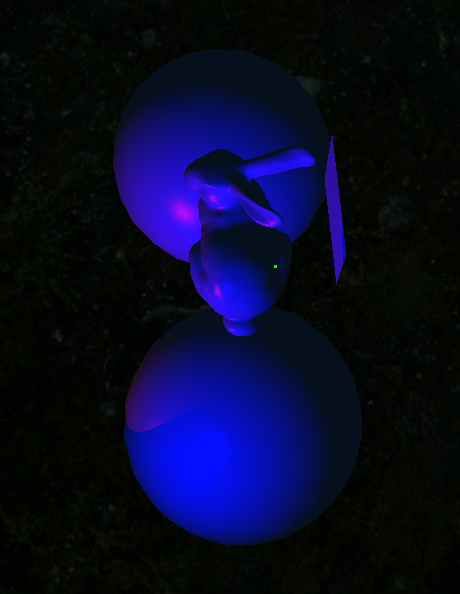
\includegraphics[width=0.48\linewidth]{3}
	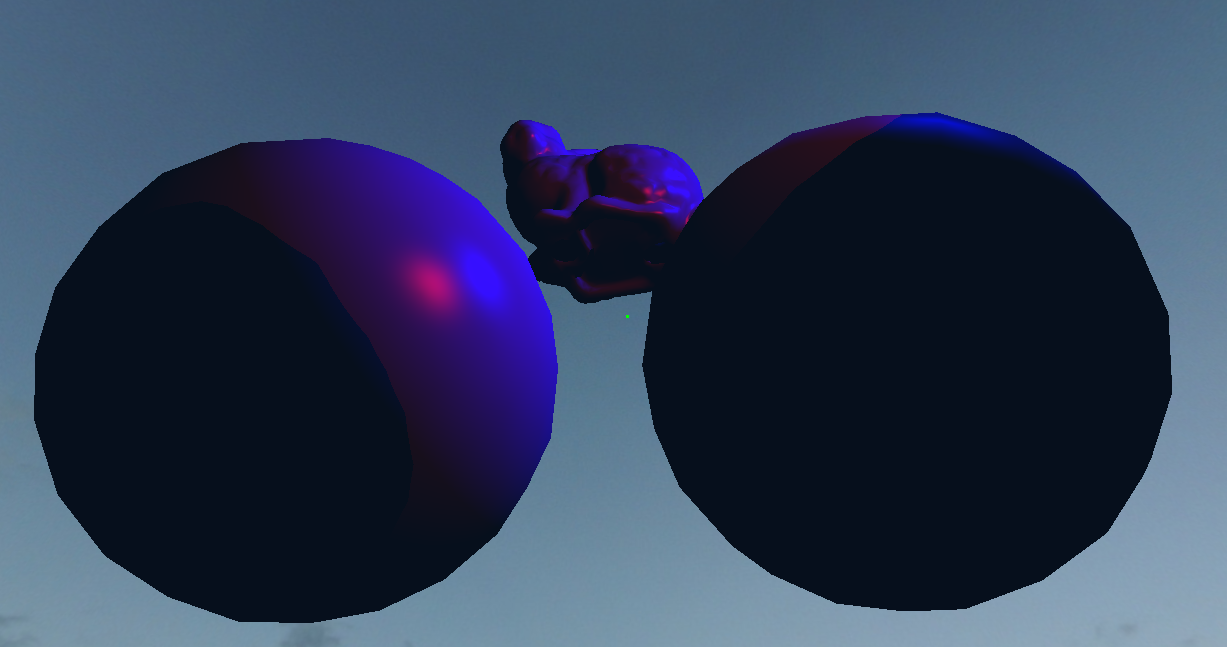
\includegraphics[width=0.48\linewidth]{4}
	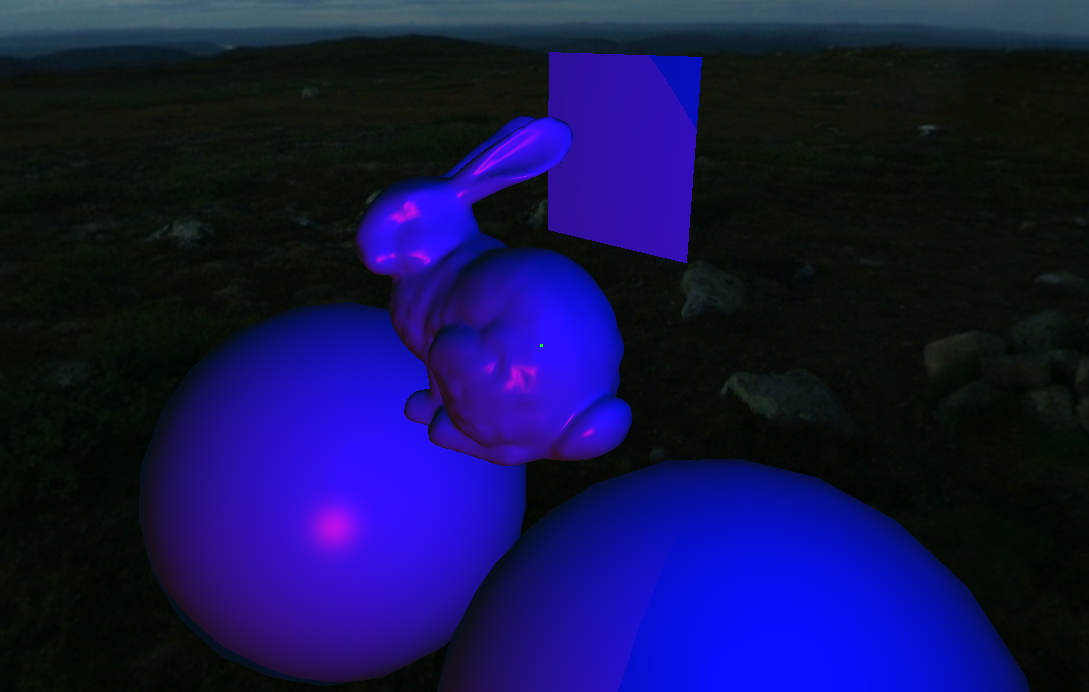
\includegraphics[width=0.48\linewidth]{5}
	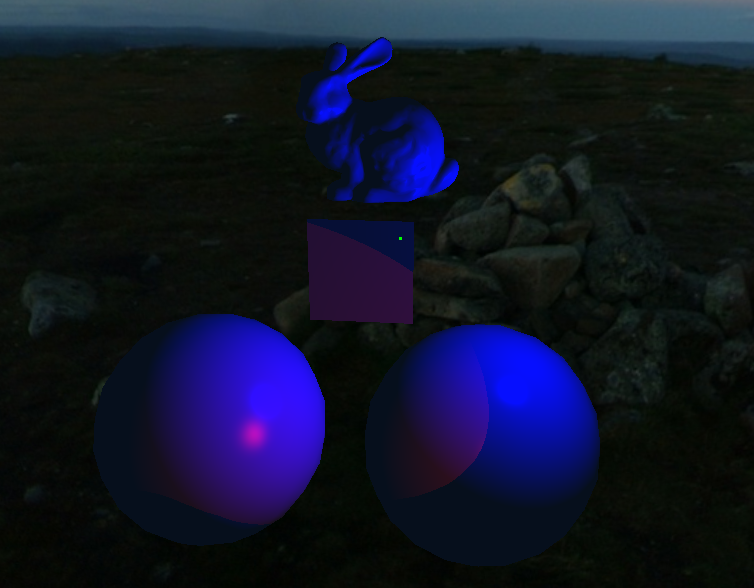
\includegraphics[width=0.48\linewidth]{6}
	\caption{phong and spotlight lightning}
\end{figure}

\end{document}
